\section{Derivation: Basic Model}
\label{section:derivation:basic_model}
\begin{enumerate}
    \item Let $\tau_s$ be the synaptic time constant of each synapse in the network. Define dimensionless time as:
    \begin{equation*}
        \xi \overset{\Delta}{=} \frac{t}{\tau_s}.
    \end{equation*}\\
    We now assume our Linear Dynamical System is expressed in dimensionless time, i.e
    
    \begin{equation}
        \label{eq:lds_dimensionless}
        \frac{dx}{d\xi} = Ax(\xi) + B c(\xi).
    \end{equation}
    
    To describe the neuron dynamics in dimensionless time, let $o(\xi) \in \mathbf{R}^{N}$ be the spike trains of N neurons composing the network with components
    \begin{equation*}
        o_j(\xi) = \sum_{k=1}^{\text{$n_j$ spikes}} \delta(\xi - \xi_{j}^{k}),
    \end{equation*}
    where $\xi_j^k$ is the time at which neuron $j$ makes its $k^{th}$ spike. 
    Define the network's estimate of the state variable as
    \begin{equation}
        \label{eq:xhat}
        \hat{x}(\xi)
        \overset{\Delta}{=} D r(\xi), 
    \end{equation}
    where $D \in \mathbf{R}^{d \times N}$ and 
    \begin{equation}
    \label{eq:rdot}
        \frac{dr}{d \xi} = -r + o(\xi).
    \end{equation}\\
    When the probability of synaptic transmission is $1$, component $r_j$ is the total received post-synaptic current (PSC) from neuron $j$ by the network estimator. 
    Define the network error as
    \begin{equation}
    \label{eq:error_def}
        e(\xi) \overset{\Delta}{=} x(\xi) - \hat{x}(\xi).
    \end{equation}
    
    \item From equations (\ref{eq:rdot}) and (\ref{eq:xhat}), we have
    
    \begin{align*}
        D \dot{r} + D r &= Do \\
        \\
        \implies \dot{\hat{x}} + \hat{x} &= Do,
    \end{align*}
    where the dot denotes derivative w.r.t dimensionless time $\xi$.

    Subtract $\dot{\hat{x}}$ from $\dot{x}$ to get $\dot{e}$:
	\begin{align*}
        \dot{e} &= \dot{x}-\dot{\hat{x}} \\
        &= \left( Ax + Bc \right) - \left( Do - \hat{x} \right) \\
        &= A\left(  e + \hat{x} \right) + Bc - Do + \hat{x} \\
        &= A e + (A + I)\hat{x} + Bc - Do \\
        &=  A e + (A + I) \left(Dr\right) + Bc - Do  \\
        \implies D^T \dot{e} &= D^T A e + D^T (A + I) \left(Dr\right) + D^T Bc - D^T Do. 
	\end{align*} 
	
The quantity $D^T e$ defines the membrane voltage of the the predictive coding framework (PCF), a precursor to this model:
$$
	v_{pcf} \overset{\Delta}{=}  D^T e.
$$
Note that the definition implies $e = D^{T \dagger} v_{pcf}$. 
The voltage dynamics are thus

\begin{align}
\label{eq:derivation_init}
\dot{v}_{pcf} 
= 
D^T A D^{T \dagger} v_{pcf} + D^T (A + I) \left(Dr\right) + D^T Bc - D^T Do,
\end{align}

where $D^{T \dagger}$ is the left pseudo-inverse of $D^T \in \mathbf{R}^{N \times d}$. The PCF thus defines a mapping between two vector spaces: the d-dimensional state space of the target system, and the N-dimensional voltage space of the spiking neural network. This mapping is visualized in figure (\ref{fig:derivation:basic_model:pcf_e_v_map}). 
\begin{figure}
    \centering
    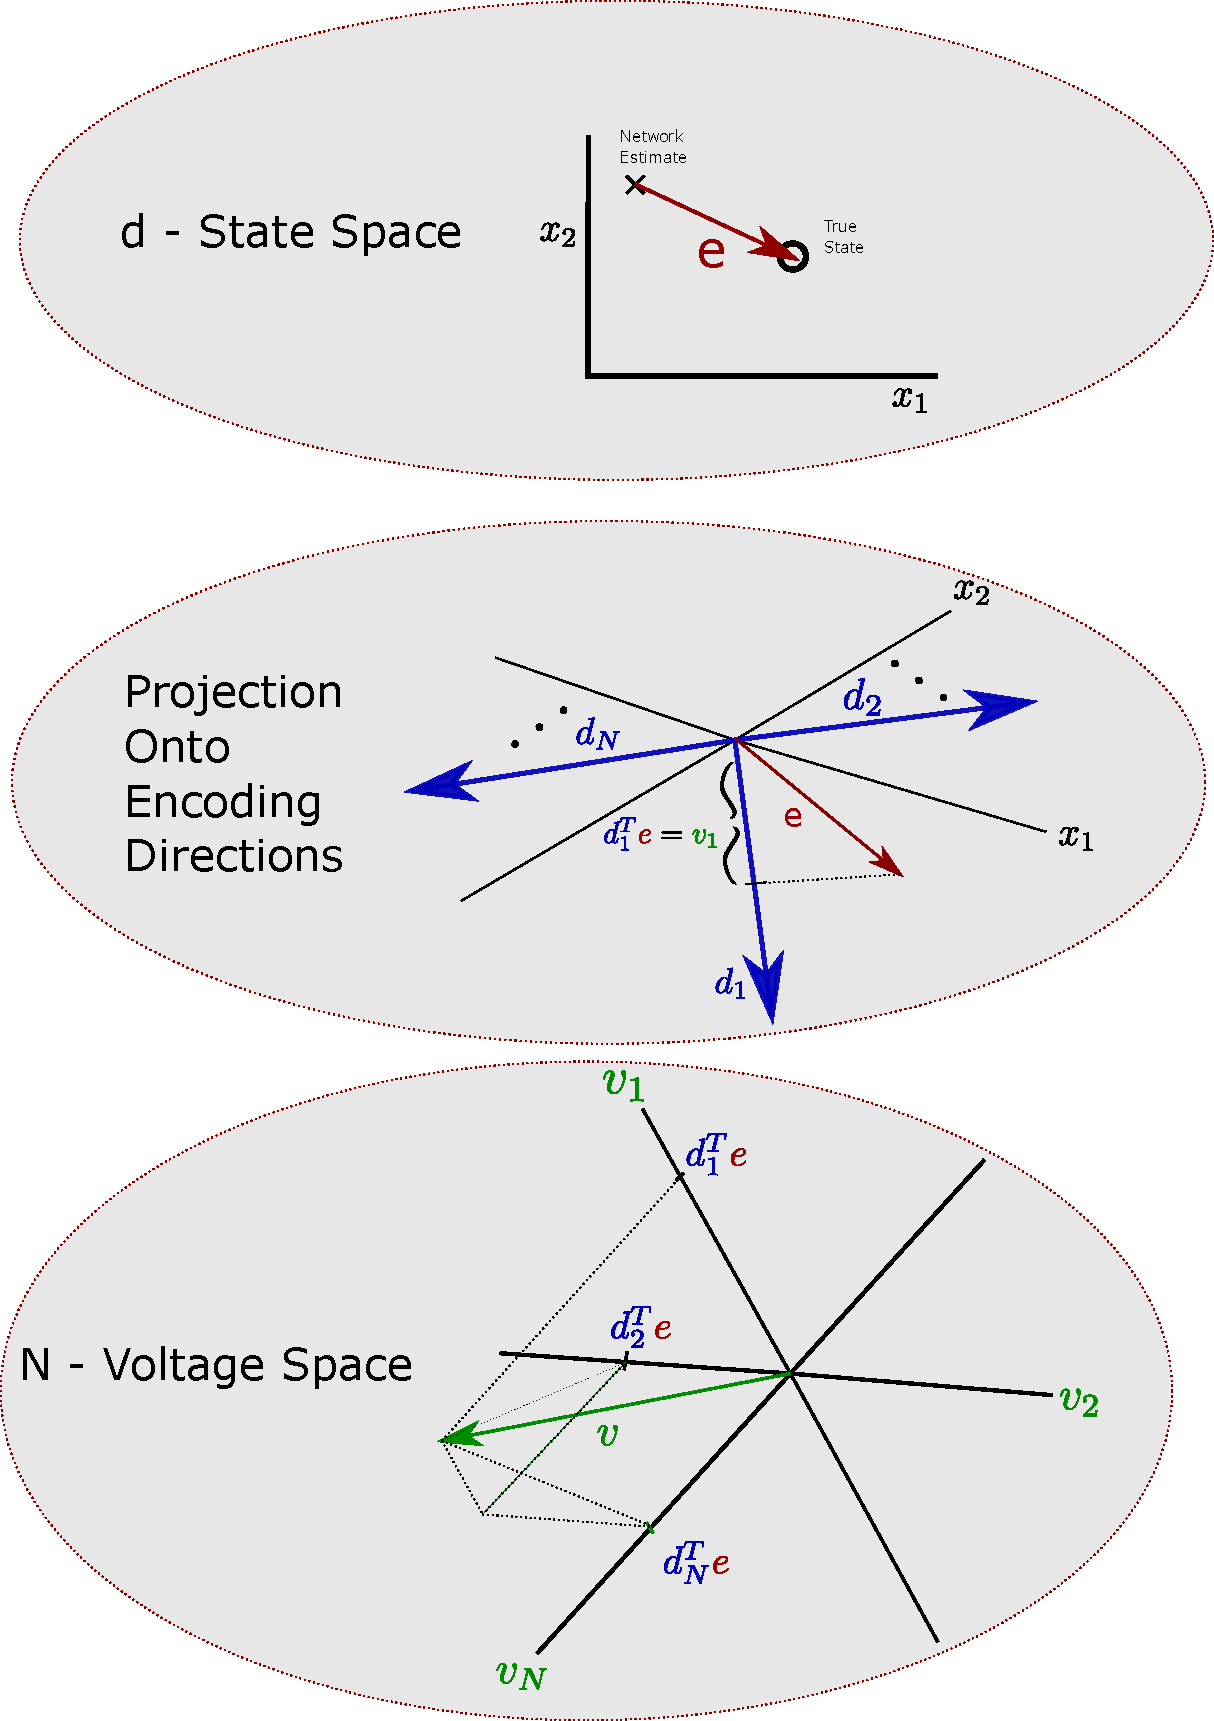
\includegraphics[scale=.703]{figures/pcf_e_v_graphic.pdf}
    \caption{Mapping Between State and Voltage Spaces: \textbf{\textit{Top:}} The estimation error $e$ is computed by comparing the decoded network estimate to the true state of the target dynamical system.  \textbf{\textit{Middle:}} The $e$ is projected onto the encoding directions of the neurons composing the network. The projection of error onto encoding direction $j$ gives the membrane voltage of neuron $j$, $v_j = d_j^T e$. \textbf{\textit{Bottom:}} The voltages form a N-dimensional vector contained in voltage space.}
    \label{fig:derivation:basic_model:pcf_e_v_map}
\end{figure}

\clearpage

\item The self-coupled network is derived by applying a change of bases.  
Assuming both $D$ and $A$ are full rank, diagonalize each to a common left basis:
\begin{align*}
    A &= \mathcal{U} \Lambda \mathcal{U}^T = \sum_{j=1}^d \Lambda_j \mathcal{U}_j \mathcal{U}_j^T,\\
    \\
    D &= \mathcal{U} \left[S \hspace{2mm} 0 \right]  V^T = \sum_{j=1}^d S_j \mathcal{U}_j  V_j^T,\\
    \\
    D^T &= V \begin{bmatrix} S \\ 0\end{bmatrix} \mathcal{U}^T = \sum_{j=1}^d S_j V_j  \mathcal{U}_j^T, \\
    \\
    D^T D  &= V \begin{bmatrix} S \\ 0\end{bmatrix} \begin{bmatrix} S & 0\end{bmatrix} V^T
     = \sum_{j=1}^d S_j^2 V_j V_j^T , 
\end{align*}
with $\mathcal{U} \in \mathbf{R}^{d \times d}$ and $V \in \mathbf{R}^{N \times N}$, and $S \in \mathbf{R}^{d \times d }$. \\
\\
To express equation (\ref{eq:derivation_init}) with the $\mathcal{U}$ and $V$ bases, first note

\begin{align*}
     D^{T} A^{-1}  &= V \begin{bmatrix} S \\ 0\end{bmatrix} \mathcal{U}^T  \mathcal{U} \Lambda^{-1} \mathcal{U}^T \\
     &= V \begin{bmatrix} S \\ 0\end{bmatrix} \Lambda^{-1} \mathcal{U}^T \\
     &= \sum_{j = 1}^{d} \frac{S_j}{ \Lambda_j} V_j \mathcal{U}_j^T,
\end{align*}\\

and

\begin{align*}
D^{T} A^{-1} D  &= V \begin{bmatrix} S \\ 0\end{bmatrix} \mathcal{U}^T  \mathcal{U} \Lambda^{-1} \mathcal{U}^T \mathcal{U} \left[S \hspace{1mm} 0 \right] V^T \\
  &= V \begin{bmatrix} S \\ 0\end{bmatrix} \Lambda^{-1} \left[S \hspace{1mm} 0 \right] V^T \\
  &= \sum_{j = 1}^{d} \frac{S_j^2}{ \Lambda_j} V_j V_j^T.
\end{align*}

Consequently, 

\begin{align}
    \label{eq:derivation_sub_svd}
    \sum_{j = 1}^{d} \frac{S_j}{ \Lambda_j} V_j \mathcal{U}_j^T \dot{e} &= 
     \sum_{j=1}^d S_j V_j  \mathcal{U}_j^T e
    +
    \sum_{j = 1}^{d} S_j^2 (1 + \Lambda_j^{-1}) V_j V_j^T r
    + 
    \sum_{j = 1}^{d} \frac{S_j}{ \Lambda_j} V_j \mathcal{U}_j^TBc 
    -
    \sum_{j = 1}^{d} \frac{S_j^2}{ \Lambda_j} V_j V_j^T o.
\end{align}


Left-multiply both sides of the preceding equation by $V_j^T$ to arrive at the system of equations

\begin{align*}
    \frac{S_j}{\Lambda_j} \mathcal{U}_j^T \dot{e} &= 
    S_j \mathcal{U}_j^T e
    +
    S_j^2 (1 + \Lambda_j^{-1})V_j^T r 
    +
    S_j \Lambda_j^{-1} \mathcal{U}_j^T B c
    -
    S_j^2 \Lambda_j^{-1} V_j^T o
    \\
    \\
    \implies 
    S_j \mathcal{U}_j^T \dot{e} 
    &= 
    S_j\Lambda_j \mathcal{U}_j^T e
    +
    S_j^2 (\Lambda_j + 1) V_j^T r 
    +
    S_j \mathcal{U}_j^T B c
    -
    S_j^2 V_j^T o,\\
\end{align*}
for $j = 1, \ldots, d$.

The preceding left-multiply has transformed the equations to the $\mathcal{U}-V$ basis. Denote the error $e$ expressed in the basis as $\epsilon$. 
\begin{align}
\label{eq:rotated_error_def}
\epsilon \overset{\Delta}{=} \mathcal{U}^T e.
\end{align}

In the $\mathcal{U}-V$ basis, left multiplication of a vector by $D^T$ is identical to scaling the first $d$ elements by the diagonal matrix $S$ and the rest by 0. The rotated voltage becomes

\begin{align}
\label{eq:rotated_voltage_def}
v \overset{\Delta}{=} S \epsilon.
\end{align}

Here, $v$ is a d vector which describes the dynamics of the d-neurons needed to implement the dynamical system. The remaining $N-d$ neurons are unused and do not contribute to the network readout at present.   \\

Denote the spike train of the rotated neurons by $\tilde{o}$. Then $\omega$ denotes the fast synaptic inhibition given by 
$$
    \omega \overset{\Delta}{=} S^2 \tilde{o}.
$$

The slow synaptic excitation is then

\begin{equation}
\label{eq:rho_dot}
    \dot{\rho} = -\rho + \omega, 
\end{equation}

where 

$$
	\rho \overset{\Delta}{=} S^2 V^T r.
$$

Similar to equation (\ref{eq:rotated_voltage_def}), $\rho$ describes a d-vector. 

The input matrix in the rotated basis is 

\begin{align}
\label{eq:rotated_input_matrix_def}
\beta \overset{\Delta}{=} \mathcal{U}^T  B.
\end{align}

Equation (\ref{eq:derivation_sub_svd}) becomes (in matrix form)

\begin{align}
\label{eq:rotated_voltage_dynamics}
    \dot{v} &= 
    \Lambda v
    +
    (\Lambda + I) \rho 
    +
     \beta c
    -
    \omega,
   \end{align}
which gives the dynamics of the rotated neuron voltages. 

There are 4 vector spaces in total: the error space which tracks the dynamical system and the network estimate, voltage space which tracks the membrane potentials, and their transformed counterparts in the $\mathcal{U}-V$ bases. Figure (\ref{fig:four_subspace_relation}) shows the relationship between these subspaces. 

\begin{figure}
\centering
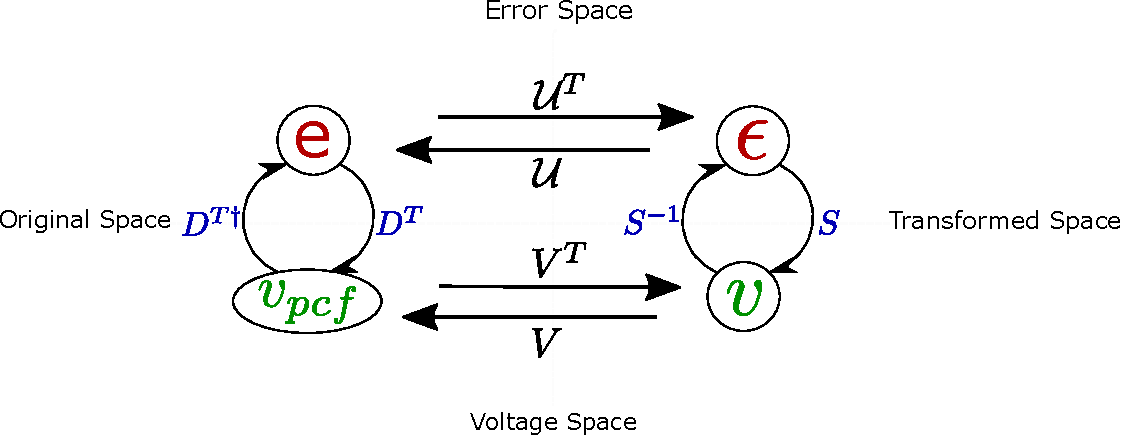
\includegraphics[width=\linewidth]{figures/ev_rotated_classic_graph}
\caption{Depiction of the relationship between original and transformed spaces and their respective error and voltage spaces. An arrow represents left multiplication by the given matrix. }
\label{fig:four_subspace_relation}
\end{figure}
   
   
\item The spike trains are chosen minimize the network estimation error
\begin{align}
    \mathcal{L}(\xi) =  || x(\xi + d\xi) - \hat{x}(\xi + d\xi) ||^2. 
\end{align}
The network greedily minimizes $\mathcal{L}$ an instant $d\xi$ ahead in time. Writing $\hat{x}$ in terms of $\omega$ and $\rho$, equations (\ref{eq:xhat}) and (\ref{eq:rotated_voltage_def}) imply 

\begin{align*}
    \hat{x} &= D r 
    \\
    \\
    &=
    \sum_{j=1}^d S_j \mathcal{U}_j V_j^T r
    \\
    \\
    &= 
    \sum_{j=1}^d S_j^{-1} \mathcal{U}_j \rho_j
    \\
    \\
    &=
    S^{-1} \mathcal{U} \rho. 
\end{align*}

If neuron $j$ does not spike, the objective is
\begin{align*}
    \mathcal{L}_{ns} = ||x - \hat{x}||^2.
\end{align*}
 
If neuron $j$ spikes at time $\xi$, then $\hat{x} \leftarrow \hat{x} + S^{-1}_j \hat{U}_j$. The objective is now
\begin{align*}
    \mathcal{L}_{sp} &= || x - (\hat{x} + \mathcal{U}_j) ||^2,\\
    \\
    &= 
    (x-\hat{x}-S^{-1}_j \mathcal{U}_j)^T (x-\hat{x}-S^{-1}_j \mathcal{U}_j)\\
    &= 
    x^T x - x^T \hat{x} - x^T S^{-1}_j \mathcal{U}_j
    - \hat{x}^T x +\hat{x}^T\hat{x} +\hat{x}^T S^{-1}_j \mathcal{U}_j
    -
    S^{-1}_j \mathcal{U}_j^T x + S^{-1}_j \mathcal{U}_j^T \hat{x} + S^{-2}_j \mathcal{U}_j^T \mathcal{U}_j
    \\
    &=
    \left(x^T x -2 x^T \hat{x} +\hat{x}^T\hat{x}  \right) + 
    2 S^{-1}_j \mathcal{U}_j^T \left( \hat{x} - x
    \right) + S^{-2}_j \mathcal{U}_j^T \mathcal{U}_j\\
    &= 
    ||x -\hat{x}|| +  2 S^{-1}_j \mathcal{U}_j^T \left( \hat{x} - x
    \right) + S^{-2}_j \mathcal{U}_j^T \mathcal{U}_j\\
    &= 
    \mathcal{L}_{ns} + 2 S^{-1}_j \mathcal{U}_j^T \left( \hat{x} - x
    \right) + S^{-2}_j \mathcal{U}_j^T \mathcal{U}_j\\
\end{align*}
 A spike occurs when it lowers the objective more than not spiking. Our spiking condition is therefore
\begin{align*}
    \mathcal{L}_{sp} &< \mathcal{L}_{ns}\\
    \\
    \implies
     2 S^{-1}_j \mathcal{U}_j^T \left( \hat{x} - x
    \right) &+ S^{-2}_j \mathcal{U}_j^T \mathcal{U}_j < 0\\
    \\
    \implies 
    S^{-1}_j \mathcal{U}_j^T \left(x -\hat{x} \right) &> \frac{S^{-2}_j \mathcal{U}_j ^T \mathcal{U}_j}{2}\\
    \\
    \implies
    S^{-1}_j \mathcal{U}_j^T e &> \frac{S^{-2}_j \mathcal{U}_j^T \mathcal{U}_j}{2}
    \\
    \\
    \implies
    \\
    \\
    S_j U_j^T e &> \frac{1}{2}
    \\
    \\
    \implies S_j \epsilon_j &> \frac{1}{2}
    \\
    \\
    \implies
    v_j &> \frac{1}{2},
\end{align*}
where the last inequality follows from equation ($\ref{eq:rotated_voltage_def}$). Thus neuron $j$ spikes when its membrane voltage $v_j$ exceeds the threshold $v_{th} = \frac{1}{2}$. 

\item Equations (\ref{eq:rotated_voltage_dynamics}) and (\ref{eq:rho_dot}) describe how we implement a network with d neurons that produces an accurate estimate $\hat{x}$ of the given target system. 


When neuron $j$ spikes, a vector $S^{-1}_j \mathcal{U}_j$ is added to the network estimate, $\hat{x}$. A spike has a strictly positive area so that the network is only able to modify its estimate by adding from a fixed set of vectors.  This restricts the space representable by the network to strictly positive state-space, or only $\frac{1}{2^d}$ of the desired state-space. To remove this restriction, we add an additional d neurons whose preferred directions $S^{-1}_j \mathcal{U}_j$ are anti-parallel to neurons $j$ for $j=1, \ldots, d$. Such vectors are required in order to allow subtraction, defined as addition of the additive inverse. Thus the number of neurons required to represent a d-dimensional system is $2d$. We update $U$, $S$, $\Lambda$ and $v_{th}$ to reflect the additional neurons:
\begin{align*}
    U &\leftarrow \left[ U \hspace{2mm} -U\right] \in \mathbf{R}^{d \times 2 d},\\
    \\
    S &\leftarrow
    \begin{bmatrix}
    S & 0 \\ 0 & S
    \end{bmatrix}
    \in \mathbf{R}^{2 d \times 2 d},\\
    \\
    \Lambda &\leftarrow
    \begin{bmatrix}
    \Lambda & 0 \\ 0 & \Lambda
    \end{bmatrix}
    \in \mathbf{R}^{2 d \times 2 d},\\
    \\
    v_{th} &\leftarrow 
    \begin{bmatrix}
    v_{th} \\ v_{th}
    \end{bmatrix} \in \mathbf{R}^{2d},
\end{align*}
and afterward recompute $\beta \in \mathbf{R}^{2 d \times d}$. 

\end{enumerate}

\subsection{Simulation of Basic Equations}
Here we simulate the above equations (\ref{eq:rotated_voltage_dynamics}) and (\ref{eq:rho_dot}) with the $N = 2d$ neurons. The parameters are
\begin{align}
\label{eq:sim_I_params}
A
&=
\ -\begin{bmatrix}  
1 & 0 \\
0 & 1
\end{bmatrix} = \mathcal{U} \Lambda \mathcal{U}^T \notag,
\\
\notag
\\
B
&=
\begin{bmatrix}  
1 & 0 \\
0 & 1
\end{bmatrix}, \notag 
\\
\notag 
\\
c(\xi) 
&=
10 \begin{bmatrix} 
cos(\frac{\pi}{4} \xi)\\
sin(\frac{\pi}{4} \xi)
\end{bmatrix} 
\\
\notag
\\
D
&=
\mathcal{U} 
\begin{bmatrix}
S & 0
\end{bmatrix}
V^T
=
\mathcal{U} 
\begin{bmatrix}
I_d & 0
\end{bmatrix}
I_N \notag,
\\
\notag 
\\
d\xi 
&= 
10^{-6}, \notag 
\\
\notag 
\\
N 
&= 
4,\notag 
\\
\notag 
\\
x(0) 
&= 
\begin{bmatrix} \frac{1}{2} & \frac{1}{2} \end{bmatrix}.\notag 
\end{align}

\begin{figure}
    \centering
    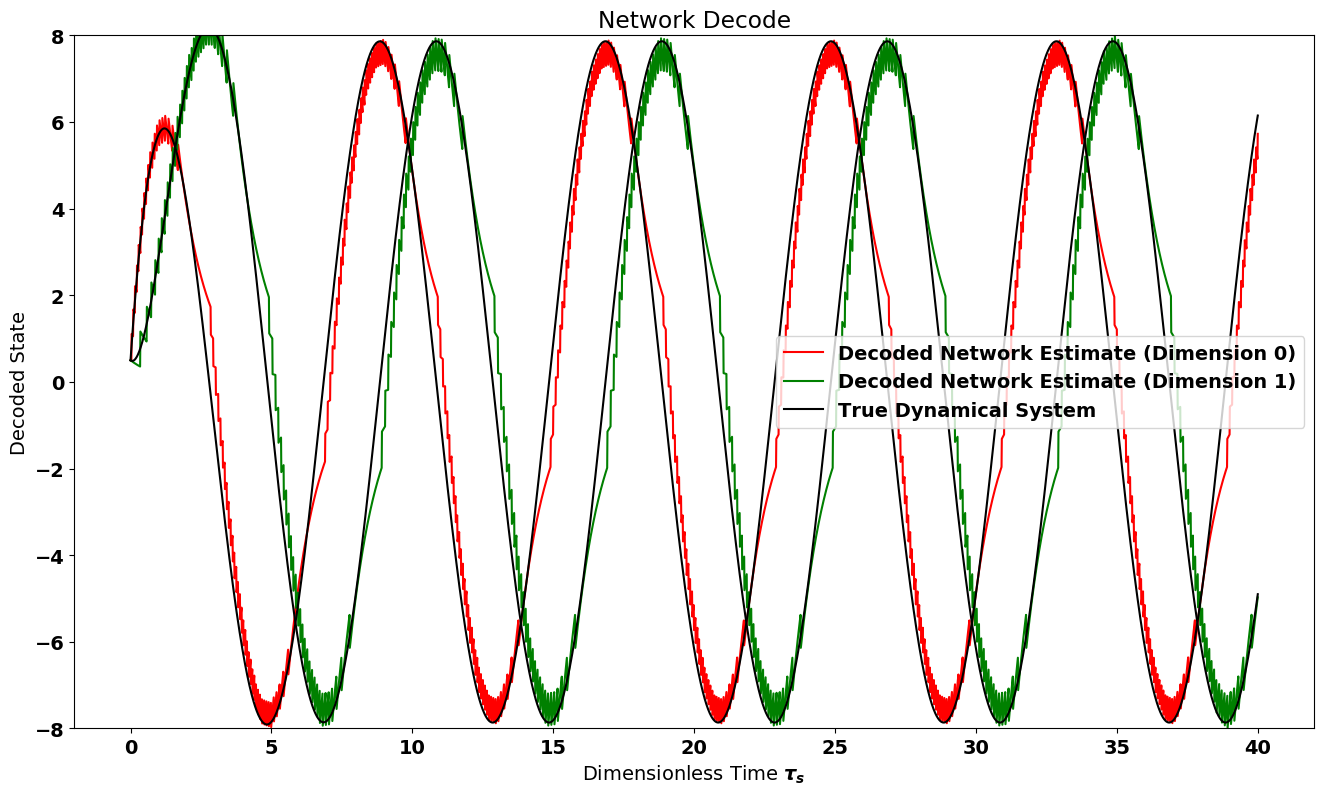
\includegraphics[width=.75\linewidth]{figures/network_decode.png}

    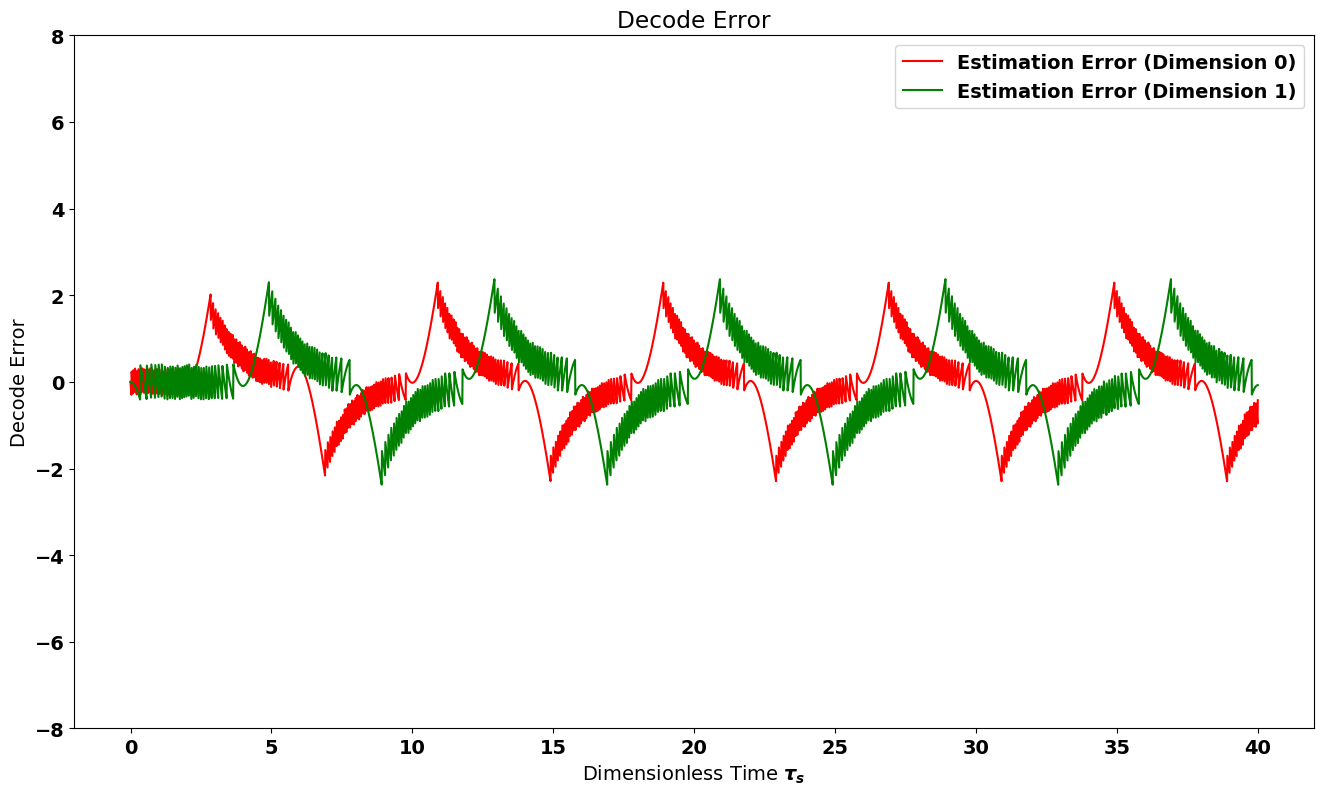
\includegraphics[width=.75\linewidth]{figures/decode_error.png}

    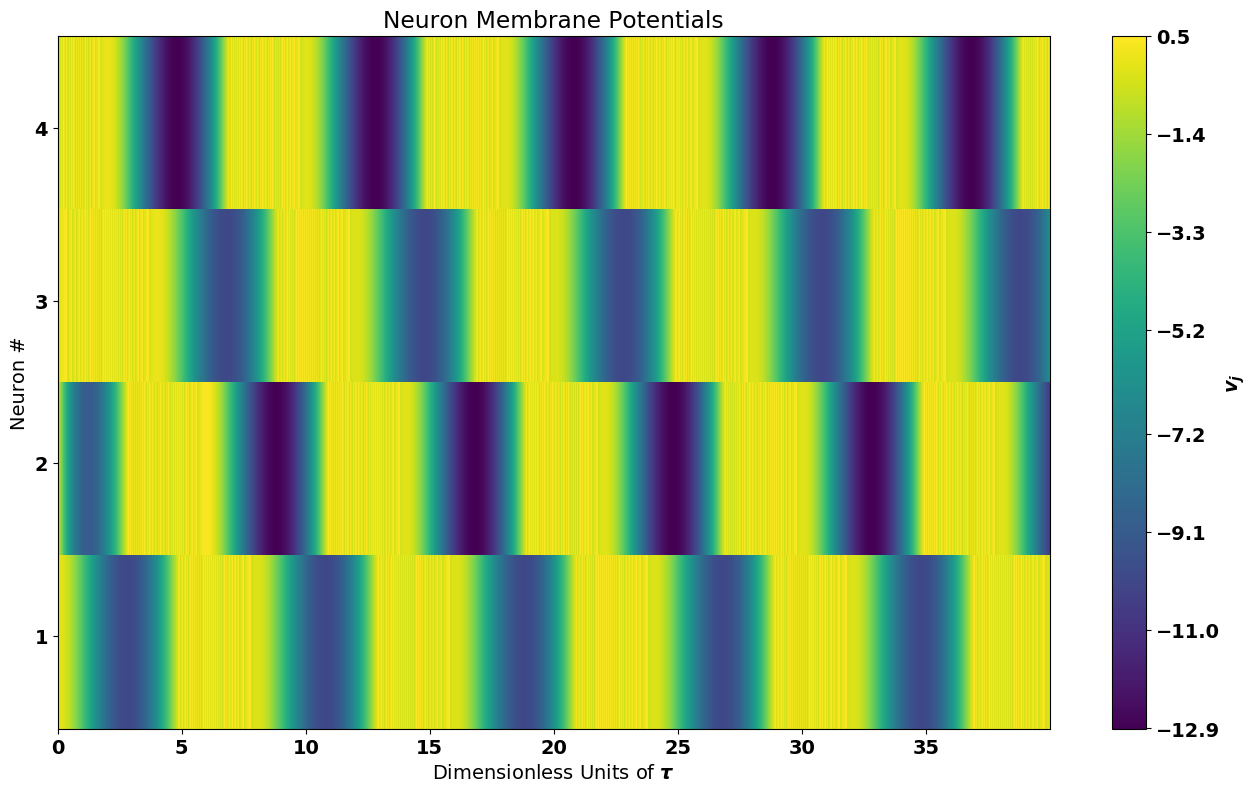
\includegraphics[width=.7\linewidth]{figures/membrane_potential_image.png}
\end{figure}

\newpage

\captionof{figure}{Simulation of equations (\ref{eq:rotated_voltage_dynamics}) and
    (\ref{eq:rho_dot}) with parameters listed in equation (\ref{eq:sim_I_params}). \textbf{\textit{Top:}} The decoded network estimate plotted alongside the target dynamical system. \textbf{\textit{Middle:}} The estimation error along each state-space dimension. \textbf{\textit{Bottom: }}The membrane potentials of the 4 neurons during the same time period.\\
    For the numerical implementation, the matrix exponential was used to integrate the continuous terms over a simulation time step. Continuous terms include all equation terms excepting the delta functions $\omega$ handled separately. After integrating over a timestep, any neuron above threshold was manually reset (action of fast inhibition). If multiple neurons are above threshold, the system is integrated backwards in time until only one neuron is above threshold before spiking. The matrix exponential was computed using a Pad\'{e} approximation via the Python package Scipy: \textit{scipy.linalg.expm()}. 
    } 
    \label{fig:Simulation_I}